\documentclass[english,11pt,twocolumn]{article}
\usepackage[utf8]{inputenc}  

\usepackage[english]{babel} 
\usepackage[T1]{fontenc}
%\usepackage{fullpage}
\usepackage[]{bbm}
\usepackage{amsfonts}
\usepackage{amsmath}
\usepackage{amssymb}
\usepackage{amsthm}
\usepackage{graphicx}
%\usepackage{pstricks}
\usepackage{float}
\usepackage{algorithm}
\usepackage{algpseudocode}

\usepackage[autolanguage]{numprint}
\usepackage[affil-it]{authblk}
%\usepackage[squaren,Gray]{SIunits}
%\usepackage{tikz}
%
%\usepackage[style=numeric,backend=bibtex]{biblatex}
\pagestyle{myheadings}


\title{Storing messages with multipartite neural cliques}
\author[]{Nissim Zerbib}
\affil{Département d'Informatique, École normale supérieure, Paris, France}

\author[]{Vincent Gripon}
\affil{Département d'Électronique, Télécom Bretagne, Brest, France}

\author{?}

\date{
	}
%

\renewcommand{\le}{\leqslant}
\renewcommand{\epsilon}{\varepsilon}
\renewcommand{\Re}{\textrm{Re}}
\renewcommand{\ge}{\geqslant}
%\newcommand{\sgn}{\textrm{le signe de }}
\newcommand{\E}{\mathcal{E}}
\newcommand{\V}{\vect{\mathcal{V}}}
\newcommand{\R}{\mathbb{R}}
\newcommand{\Z}{\mathbb{Z}}
\newcommand{\z}[1]{\Z/#1\Z}
\renewcommand{\P}{\mathbb{P}}
\newcommand{\Q}{\mathbb{Q}}
\newcommand{\N}{\mathbb{N}}
\newcommand{\C}{\mathbb{C}}
\newcommand{\U}{\mathbb{U}}
\newcommand{\f}{\widehat{f}}
\newcommand{\e}[1]{e^{-2 \pi i #1}}
\newcommand{\ex}[1]{e^{2 \pi i #1}}
\renewcommand{\L}[1]{L^{#1} (\R )}
\newcommand{\leg}[2]{\left(\dfrac{#1}{#2}\right)}

\newcommand{\vect}[1]{\overrightarrow{#1}}
\newcommand{\disp}[1]{\displaystyle{#1}}

\setcounter{secnumdepth}{3} %pour la numérotation subsubsection
\setcounter{tocdepth}{3} %pour la numérotation dans la table de matières
\renewcommand{\theenumi}{\roman{enumi})}
\renewcommand{\thepart}{\Alph{part}}
%\renewcommand{\thechapter}{\arabic{chapter}}
\renewcommand{\thesection}{\Roman{section}}
\renewcommand{\thesubsection}{\arabic{subsection}}
\renewcommand{\thesubsubsection}{\alph{subsubsection}}

\newcommand*\Let[2]{\State #1 $\gets$ #2}
\algrenewcommand\algorithmicrequire{\textbf{Input:}}
\algrenewcommand\algorithmicensure{\textbf{Output:}}

\newcommand{\fonction}[5]{\begin{array}{cllll}
#1 & : & #2 & \longrightarrow & #3 \\
&    & #4 & \longmapsto & #5 \end{array}}
\newcommand{\fonc}[3]{\begin{array}{lllll}
#1: & #2 & \mapsto & \displaystyle{#3}\end{array}}
\newcommand{\app}[3]{
	#1 : #2 \mapsto \displaystyle{#3}}
\newcommand{\fonct}[3]{\begin{array}{ccccc}
#1: & #2 & \longrightarrow & \displaystyle{#3}\end{array}}
\newcommand{\pent}[1]{\lfloor #1 \rfloor}

% Le point-virgule bien espacé
\newcommand{\pv}{\ensuremath{\, ; }}
% Les intervalles
   % fermé - fermé
   \newcommand{\interff}[2]{\ensuremath{\left[ #1 \pv #2 \right]}}
   % fermé - ouvert
   \newcommand{\interfo}[2]{\ensuremath{\left[ #1 \pv #2 \right[}}
   % ouvert - fermé
   \newcommand{\interof}[2]{\ensuremath{\left] #1 \pv #2 \right]}}
   % ouvert - ouvert
   \newcommand{\interoo}[2]{\ensuremath{\left] #1 \pv #2 \right[}}


\theoremstyle{definition}
\newtheorem{theoreme}{Theorem}
\renewcommand{\thetheoreme}{\arabic{section}.\arabic{theoreme}}
\providecommand{\keywords}[1]{\textbf{Index terms---} #1}

\newcommand{\comp}[3]{\left\{
	#1\,;\, #1\in #2 \, /\, #3
	\right\}}
\newcommand{\param}[2]{\left\{
	#1\, /\, #2
	\right\}}


\begin{document}

	\maketitle

	 \begin{abstract}
	 	We extend recently introduced associative memories based on clustered cliques to multipartite cliques. We propose a variant of the classic retrieving rule. We study its performance relatively to the former one for retrieving partially erased or corrupted messages. We provide both analytical and simulation results showing improvements in both networks capacities and resilience. We compute asymptotic capacities of these networks.
	 \end{abstract}
	 
	\keywords{associative memory, error correcting code, cliques, multipartite cliques, neural networks}
	
	\section{Introduction}
	
	
	
	\section{Networks of neural cliques}
		
	\subsection{Learning messages}
		
	Let $\mathcal{M}$ be a set of messages of length $c$ over the alphabet $\mathcal{A} = \{1, 2, \hdots, {l \choose a}\}$ and $m = | \mathcal{M} |$. Messages in $\mathcal{M}$ are stored in an undirected unweighted graph, or neural network, of $c \cdot l$ vertices or neurons. 
	
	Each message $x = (x_i)_{1 \le i \le c}$ is mapped to $y = (y_i)_{1 \le i \le c}$ where $y_i$ is the binary representation of the $x_i$-th $a$-combination of $l$ elements (the mapping doesn't matter as long as it is fixed).
	
	Storing a message $x$ in the network amounts to consider the network in state $y$, that is for all $1 \le j \le l$ and $1 \le i \le c$, the neuron $j$ in the cluster $i$ is activated if and only if $y_{i,j} = 1$ ; then adding all connections between activated neurons excepting for neurons sharing the same cluster. Thus we obtain a multipartite clique between activated neurons representing a message. The parameter $a$ describing the number of activated neurons per cluster will be called number of activities.
		
	\subsection{Retrieving messages}	
		
		Retrieving messages occurs by message passing.		
		
		\subsubsection{The "winner takes all" rule}
		
		take only maximum score
	
		\subsubsection{The "$w$-winners take all" rule}
		

		To fully exploit the local regularity of the code (constant weight of $w$), we make a small modification the classic retrieving rule	by keeping activated all neurons that achieve a score equal or greater than the score appearing in $w$-th position in the ordered array of scores (where $w$ is a positive integer parameter)
		
		%$a$-rank
		
		Although it is a less biologically plausible rule, it has the same algorithmic complexity, since selecting the $w$-th element in an array of $n$ elements is $O(n)$ in complexity.
		
		Intuitively the choice $w = a$ is optimal (it it is the most natural with $w = 1$).
		The following is a description of the algorithm\footnote{No optimizations are described here (early stopping etc.)} :
		\begin{algorithm}
		\caption{$w$-sum of sum \label{asumsum}}
		
		\begin{algorithmic}[1]
		\Require{$v$ a binary array of length $n = c\cdot l$, $W$ the binary weight matrix representing the network}
		\Procedure{Sum of sum}{$v, W, \gamma, S, w$}
		%\Statex
		\For{$s$ from $1$ to S}
		\State $s \gets \gamma v + W v$
		\For{$i$ from $1$ to $c$}
			\Let{treshold}{Select(s[$i$], $w$)} \Comment{Select(t, w) returns the element that would be in rank $w$ if the array t was sorted}
			\For{$j$ from $1$ to $l$}
			\Let{$v[i][j]$}{$s[i][j]$ $\ge$ treshold}
			\EndFor
		\EndFor
		\EndFor
		%\State\Return v
		\EndProcedure
		\end{algorithmic}
		\end{algorithm}

	\section{Retrieval performance}	
	

	\subsection{Retrieving partially erased messages}		
		
	\subsubsection{Analytical result}
		
	%number of neurons per cluster $l$
	
	%number of clusters $c$
	
	%number of erased clusters $c_e$
	
	%number of messages : $m$
	
	%number of activities per cluster : $a$
	
	%density : $d$
	
	%edge : $(i, j)$
	Suppose we are trying to recover a message where $c_e$ clusters have been erased.
	
	As the probability for $i$ and $j$ to be active in their respective clusters for one message is $\frac{a}{l}$ providing messages are identically distributed, it follows that the probability for the edge $(i,j)$ of not being added in the network for one message is $1 - \left(\frac{a}{l}\right)^2$. Since messages are independent, the density $d$, which is the probability for an edge to be in the network, can be expressed like this :
	
	\begin{align}
		\label{formula_density}
		d = 1 - \left( 1 - \left(\frac{a}{l}\right)^2 \right)^m 
	\end{align}		
	
	Thanks to the memory effect $\gamma$, activated neurons in a non-erased cluster stay activated and are the only ones doing so in their cluster. For neurons in erased clusters, the maximum attainable score is $a(c - c_e)$. Neurons corresponding to the original message achieve this score. Besides the probability for a neuron $v$ to achieve the maximum score in such a cluster, that is to mean $a(c-c_e)$ is $d^{a(c-c_e)}$.
	
	%probability for a vertex $v$	not to achieve the maximum : $1 - d^	{a(c-c_e)}$
	
	Since neurons representing messages are independent (as messages are themselves independent), the probability for none of the vertices of one erased cluster, excepting the correct ones, to achieve the maximum is $\left(1 - d^	{a(c-c_e)}\right)^{l-a}$.
	
	Scores in clusters being also independent, the probability for none of the vertices in any erased cluster, excepting the correct ones, to achieve the maximum in their respective clusters is $\left(1 - d^	{a(c-c_e)}\right)^{c_e(l-a)}$.
	
	Whence error rate in retrieving messages is : 
	\begin{align}	
	P_{err} = 1 -	\left(1 - d^	{a(c-c_e)}\right)^{c_e(l-a)} 
	\end{align}	 
	
	We define the efficiency of the network relatively to the hardness of the problem (how much it is efficient compared to a perfect associative memory). A perfect associative memory would use exactly the same number of bits than the original messages and recover messages by maximum likelihood (ambiguities causing errors). Efficiency is the amount of information retrieved divided by the hardness of the problem.
	
	The network is a binary symmetric matrix with null diagonal and can therefore be stored in memory as $\frac{c(c-1) l^2}{2}$ bits. Since messages are not stored in an ordered fashion, the information stored is the set of messages, thereby it amounts to $\log_2(\frac{({l \choose a}^c)^m}{m!}) \approx m(c \log_2{l \choose a } - \log_2(m) + 1) $. The information effectively stored in the network is $P_{retrieve} \times m  \frac{2 \left(c \log_2{l \choose a } - \log_2(m) + 1 \right)}{c(c-1)l^2}$.
	
	Ambiguities would occur in a perfect associative memory if at least two messages were identical over non-erased letters. The probability it doesn't happen is $ (1-{l \choose a}^{c - c_e})^{m-1}$.
	
	
	$\eta_m = P_{retrieve} m  \frac{2 \left(c \log_2{l \choose a } - \log_2(m) + 1 \right)}{c(c-1)l^2} \times (1-(\frac{1}{{l \choose a}})^{c - c_e})^{-(m-1)}$
	%\frac{c}{(c-c_e) \log_2{l \choose a }}
	
	The maximum information that can be stored in the network is therefore $\eta = \max_x \eta_x $.
	
	\subsubsection{Simulations}
		Theoretical and empirical densities match very closely, see Figure \ref{densiteth}. %gap of theoretical density with density in simulations : under $1$ percent, 
		
		
		
		Simulations agree with the analytical results for error rate, see Figure \ref{erasuresth}.
	

	For one iteration (for erasures, not for errors), "winner takes all" is the same as "$a$-winners take all".
	
	For multiple iterations $a$-winners take all is a significant improvement.
	%The variant of the rule significantly improves the retrieval rate over multiple iterations. (For one iteration, is is the same as taking only maximum scores.)
	
	%See Figure \ref{erasuresth}	
	
		
	\begin{figure}[!htb]
		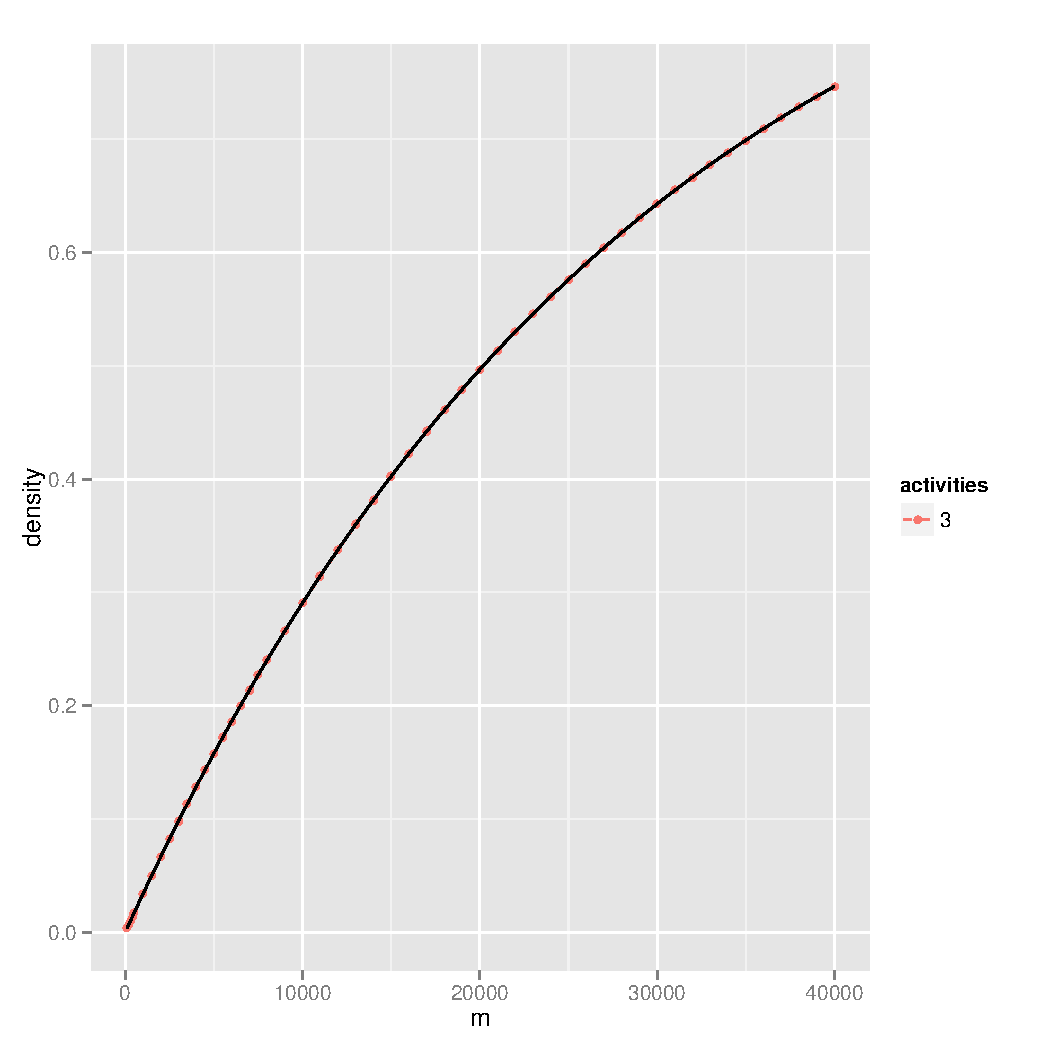
\includegraphics[width=8.5cm]{Courbes/densiteexemple.pdf}
		\caption{Theoretical and empirical densities}
			\label{densiteth}
	\end{figure}
	
	
	\begin{figure}[!htb]
		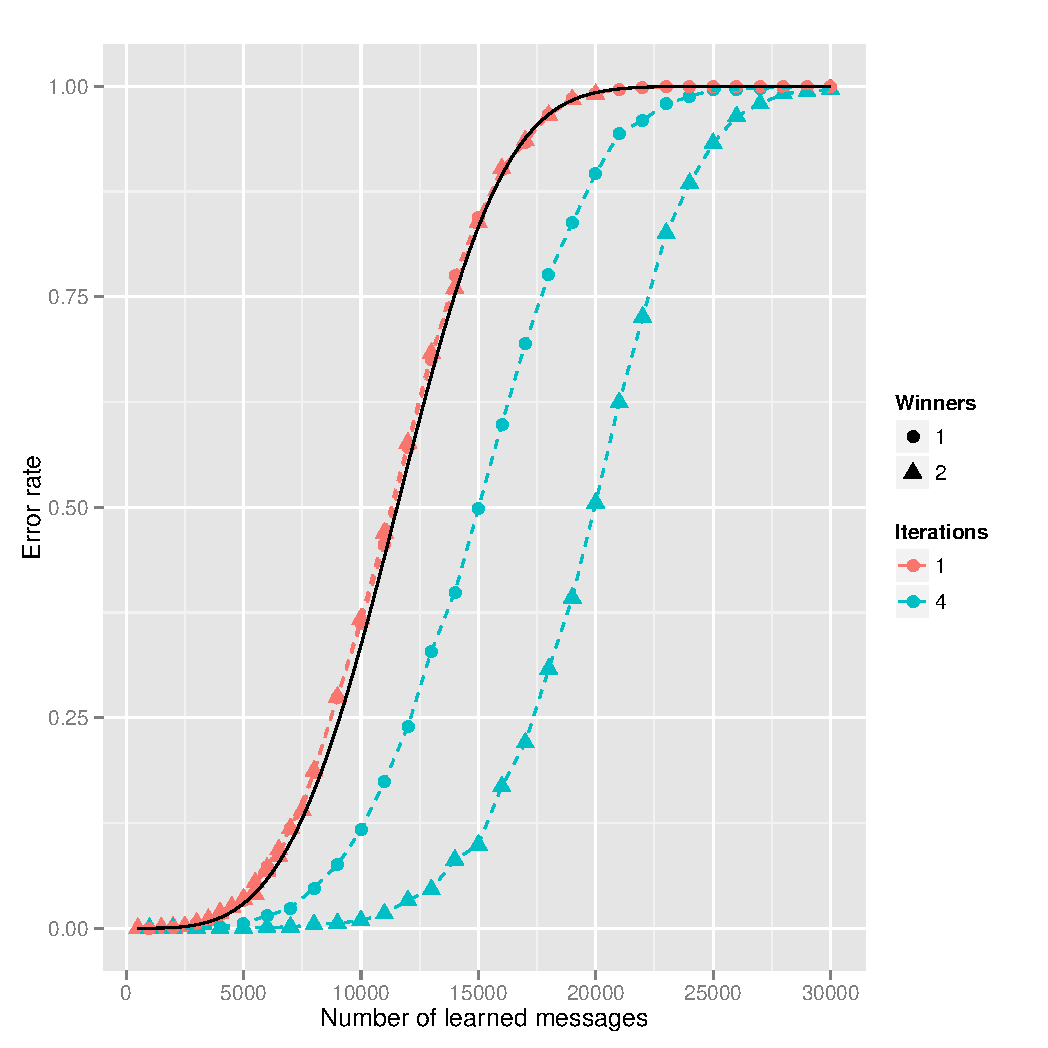
\includegraphics[width=8.5cm]{Courbes/remplacement_figure2g1} %{comparaison_regles_pool5_a2c4l512e2}
		\caption{2 activities per cluster, 4 clusters, 512 neurons per cluster, two erasures, each point is the mean of 5 networks with 1000 sampled messages, analytical result in continuous black}
			\label{erasuresth}
		\end{figure}
		
		Figure \ref{comperth} shows improvements in capacities over unipartite cliques network. The more the problem is difficult, the more redundancies introduced by multipartite cliques are useful.
		
		\begin{figure}[!htb]
		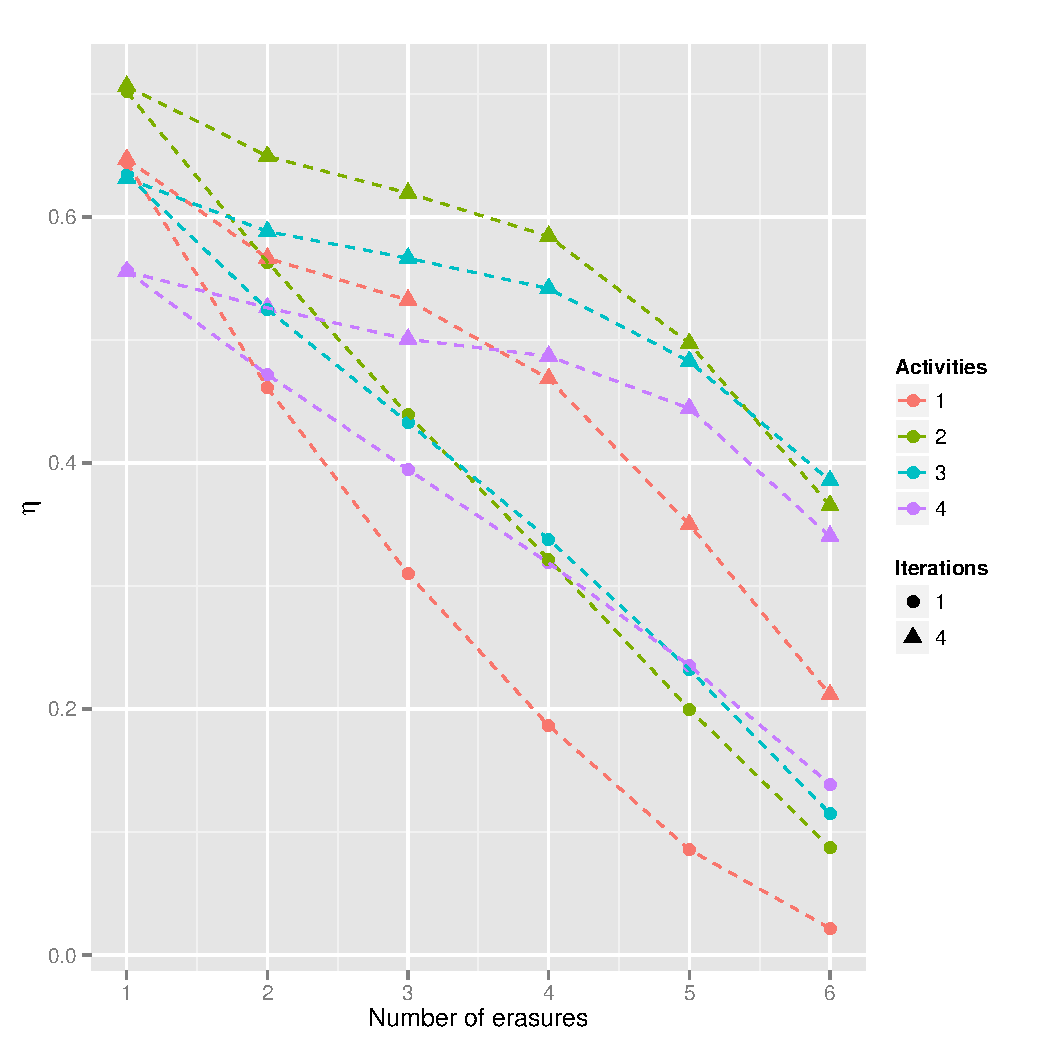
\includegraphics[width=8.5cm]{Courbes/5portant_erasures_c8l256}
		\caption{Comparison between different number of activities per cluster :  8 clusters, 256 neurons per cluster, 1000 sampled messages, pools of 5}
		\label{comperth}
	\end{figure}
%	
%	\newpage
%	$\,$
%	\newpage
%	$\,$
%	\newpage
	
	\subsection{Retrieving corrupted messages}
	
	\subsubsection{Analytical result}	
%	Formula for errors instead of erasures : 
%	
%	gc : good (à remplacer par right/wrong ?) neuron in correct cluster
%	
%	ge : good neuron in erroneous cluster
%	
%	abe : bad activated neuron in erroneous cluster
%	
%	be : others bad (à remplacer par wrong ou incorrect etc.) neurons in erroneous cluster
%	
%	bc : bad neuron in correct cluster
	Messages can be corrupted, our models for errors is : fix $c_e$ the number of erroneous clusters, we draw at random $c_e$ clusters and in each of these draw at random, uniformly, a new letter in the alphabet that will replace the old one (it could be the same).
	
	Knowing the density of the network, which follows formula (\ref{formula_density}), we can compute the laws of probabilities for scores achieved by different type of neurons in different clusters. We can divide neurons in 5 groups. Subscript $g$ will indicate a neuron being part of the message (it should be activated), subscript $b$ the contrary (the neuron should not be activated). Subscript $a$ means the neuron is already activated. Subscript $c$ corresponds to a correct cluster, $e$ to an erroneous cluster.
	Correct neurons in uncorrupted clusters achieve at least a score of $a(c-c_e - 1) + \gamma$. 
	Being connected to a given activated neuron in a corrupted cluster occurs with probability $d$, since errors are identically distributed. Moreover corrects neurons see their scores shift, as do all activated neurons respectively thanks to being part of the original message and the memory effect $\gamma$. We can express those probability laws as : 
	For example an \textbf{a}ctivated \textbf{g}ood neuron in a \textbf{c}orrect cluster starts with a base score of $ a(c - c_e - 1) + \gamma$. The probability it has to be connected to a random activated neuron in an erroneous cluster is $d$. Thereby its law is :
	
	%$P(n_{agc} = (c - c_e - 1) + \gamma + x) = {c_e \choose x} d^x (1-d)^{ce-x}$
	$P(n_{agc} = a(c - c_e - 1) + \gamma + x) = {a c_e \choose x} d^x (1-d)^{a ce-x}$
	
	Correct neurons in corrupted clusters achieve at least a score of $a(c - c_e)$. 
	$P(n_{ge} = a(c - c_e) + x) = {a (c_e - 1) \choose x} d^x (1-d)^{a (c_e - 1)-x}$
	
	%$P(n_{ge} = (c - c_e) + x) = {c_e - 1 \choose x} d^x (1-d)^{c_e-1-x}$
	
	Activated neurons benefits of the memory effect $\gamma$ :	\\
	$P(n_{abe} = \gamma + x) = {a(c - 1) \choose x} d^x (1-d)^{a(c-1)-x}$
	%$P(n_{abe} = \gamma + x) = {c - 1 \choose x} d^x (1-d)^{c-1-x}$
	
	
	%$P(n_{be} = x) = P(n_{bc} = x) = {c - 1 \choose x} d^x (1-d)^{c- 1 -x}$
	Finally $P(n_{be} = x) = P(n_{bc} = x) = {a(c - 1) \choose x} d^x (1-d)^{a(c- 1) -x}$	
	
	A message is retrieved after one iteration, if and only if correct neurons achieve strictly the best scores.	
	
%	\begin{align}
%	P_{retrieve} = \left [ \sum_{n = 1}^{c-1+\gamma} P(n_{agc} = n) \left [ \sum_{x=0}^{n-1} P(n_{bc} = x) \right]^{l-1} \right ]^{c - c_e} \\ \times \left [ \sum_{n = 1}^{c-1+\gamma} P(n_{ge} = n) \left [ \sum_{x=0}^{n-1} P(n_{bc} = x) \right]^{l-2} \left [ \sum_{x=0}^{n-1} P(n_{abc} = x) \right] \right ]^{c_e}
%	\end{align}
	
%	\begin{align*}
%	P_{retrieve} = \left [ \sum_{n = 1}^{c-1+\gamma} P(n_{agc} = n)  P(n_{bc} < n)^{l-1} \right ]^{c - c_e} \\ \times \left [ \sum_{n = 1}^{c-1+\gamma} P(n_{ge} = n) P(n_{bc} < n)^{l-2} P(n_{abc} < n) \right ]^{c_e}
%	\end{align*}

	
	%à changer : prendre en compte les $a$ neurones activés : problème des recouvrements !! on est trop optimiste si grand nombre d'activités (ou pessimiste ?)
	
	
	
	


	
	\begin{align}
	&P_{retrieve} = \left [ \sum_{n = 1}^{a(c-1) + \gamma} \left [ \sum_{k = 1}^{a} { a \choose k }   P(n_{agc} = n)^k P(n_{agc} > n)^{a-k} \right ] P(n_{bc} < n)^{l-a} \right ]^{c - c_e}\\ 
	 &\times \left [ \sum_{n = 1}^{a(c-1) +\gamma} \left[ \sum_{k = 1}^a { a \choose k } P(n_{ge} = n)^k P(n_{ge} > n)^{a-k} \right ] P(n_{be} < n)^{l-2a} P(n_{abe} < n)^a \right ]^{c_e}
	\end{align}
	

%	To be really precise : (ne pas oublier de tenir compte changement des lois, formule inexacte pour l'instant)
%	\begin{align*}
%	&P_{retrieve} = \left [ \sum_{n = 1}^{a(c-1) + \gamma} \left [ \sum_{k = 1}^{a} { a \choose k }   P(n_{gc} = n)^k P(n_{gc} > n)^{a-k} \right ] P(n_{bc} < n)^{l-a} \right ]^{c - c_e}\\ 
%	 &\times \left [ \sum_{y = 0}^a \left( \frac{{l-y \choose a} - \sum_{z = y+1}^{a} {l-z \choose a }}{{l \choose a}}\right)\sum_{n = 1}^{a(c-1) +\gamma} \left[ \sum_{k = 1}^a { a \choose k } P(n_{ge} = n)^k P(n_{ge} > n)^{a-k} \right ] P(n_{bc} < n)^{l-a - y} P(n_{abc} < n)^{a - y} \right ]^{c_e}
%	\end{align*}	
	
	$P_{err} = 1 - P_{retrieve}$	

	
	
	\newpage
	$\,$
	\newpage	
	
	\subsubsection{Simulations}
	See Figure \ref{corruptth} compares the two rules.
	"$a$-winners take all" better than "winner takes all" with errors instead of erasures, even for one iteration.
	
	\begin{figure}[!htb]
		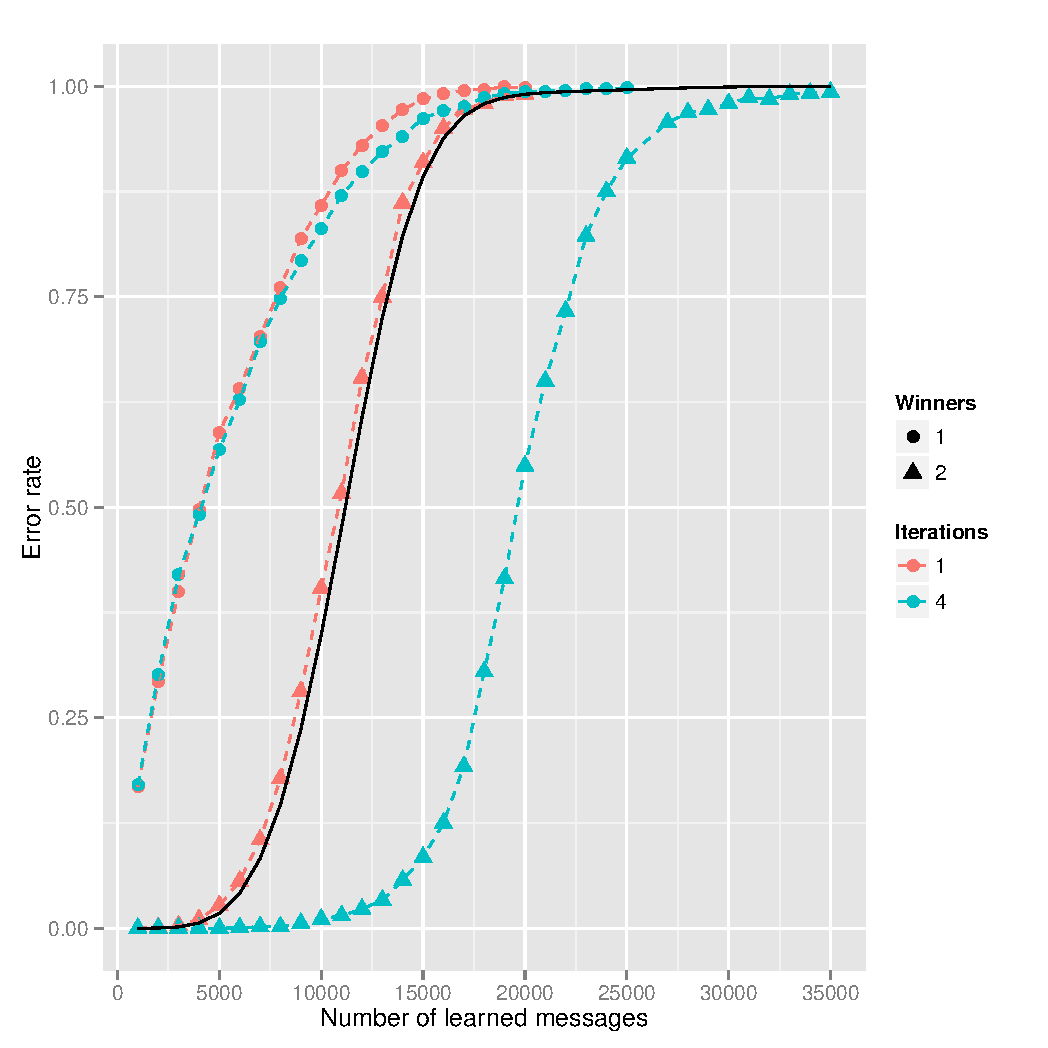
\includegraphics[width=8.5cm]{Courbes/remplacement_figure3g1}
		\caption{2 activities per cluster, 4 clusters, 512 neurons per cluster, one erroneous cluster, each point is the mean of 5 networks with 1000 sampled messages, analytical result in continuous black}
		\label{corruptth}
	\end{figure}
		
		$\eta_m = P_{retrieve} m  \frac{2 \left(c \log_2{l \choose a } - \log_2(m) + 1 \right)}{c(c-1)l^2} \times \left [\sum_{k = c_e+1}^{c} \left (1-\frac{1}{{l \choose a}} \right )^k \left (\frac{1}{{l \choose a}} \right )^{c-k} \right ] ^{-(m-1)}$
		
		

	
	\section{Resilience}
	%Spéculations en Français 
	%Peut-être un intérêt pour cluter based associative memories build from unreliable storage : si une arête porte moins d'info, on peut peut-être en supprimer plus (mais rajout ?!)
	
	As information is shared accross connections with multiple activated neurons per cluster, they are more resilient to network damages (for one message information is carried by $a^2 {c \choose 2}$ edges. $v_c$ will indicate a correct neuron that should be activated, $v$ the other type of neurons.
	
	Our deviation model is drawn from \cite{LedGriRabGro20145}\footnote{Compared to this article, we do not draw at random a letter in case of ambiguity, which hurts performance a bit.}.
	
	$P(n_{v_c} = x + \gamma ) = {a (c_k-1) \choose x} (1-\psi)^{x} \psi ^ { a (c - c_e -1) - x }$	
	
	$P(n_{v_c} = x) = {a c_k \choose x} (1-\psi)^{x} \psi ^ { a (c - c_e) - x }$
	
	$P_+ = \psi (1 - d) + (1 - \psi) d$
	
	$P(n_v = x) = {a c_k \choose x} P_+^x (1-P_+)^{a c_k -x }$

	% À corriger avec sommes multiparties
	$P(\mbox{no other vertex activated in this cluster})= \sum_{n_0 = 1}^{a (c - c_e)} P(n_{v_c} \ge n_0)^a \left [ \sum_{x = 0}^{n_0 - 1} P(n_v = x) \right]^{l-a}$
	
	% Approx : ?! $P(\mbox{no other vertex activated in any cluster})=  \left ( \sum_{n_0 = 1}^{a ( c - c_e)} P(n_{v_c} \ge n_0)^a \left [ \sum_{x = 0}^{n_0 - 1} P(n_v = x) \right]^{l-a } \right)^{c_e}$
	
	Sans tenir compte du choix au hasard si plus sont activés. Pour une itération $\gamma = \infty$. Pour plusieurs $\gamma = 1$.
	
		a priori for noise on edges :

	$P(\mbox{no other vertex activated in this cluster})= \sum_{n = 1}^{a (c - c_e)} \left [ \sum_{k = 1}^{a} { a \choose k }   P(n_{v_c} = n)^k P(n_{v_c} > n)^{a-k} \right ] P(n_v < n)^{l-a}$%[ \sum_{x = 0}^{n - 1} P(n_v = x) \right]^{l-a }$
	
	$P(\mbox{no other vertex activated in any cluster})=  \left ( \sum_{n = 1}^{a ( c- c_e)} \left [ \sum_{k = 1}^{a} { a \choose k }   P(n_{v_c} = n)^k P(n_{v_c} > n)^{a-k} \right ] \left [ \sum_{x = 0}^{n - 1} P(n_v = x) \right]^{l-a } \right)^{c_e}$	
	
	\newpage
	%$\,$
	%\newpage
	\begin{figure}[!htb]
		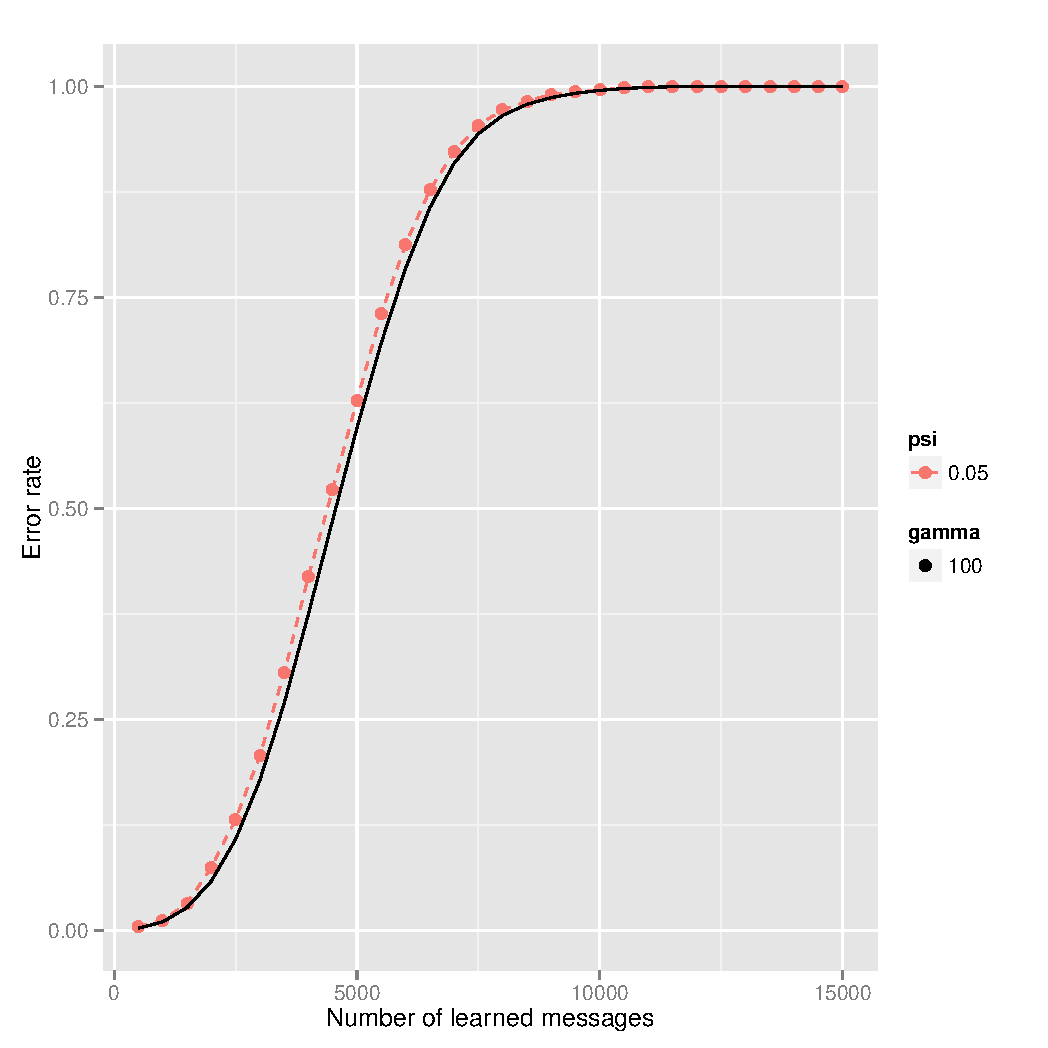
\includegraphics[width=8.5cm]{Courbes/thpsi_c8l256e4}
		\caption{2 activities per cluster, 8 clusters, 256 neurons per cluster, 4 erasures, each point is the mean of 10 networks with 1000 sampled messages, analytical result in continuous black}
		\label{psith}
	\end{figure}
	
	\begin{figure}[!htb]
		
		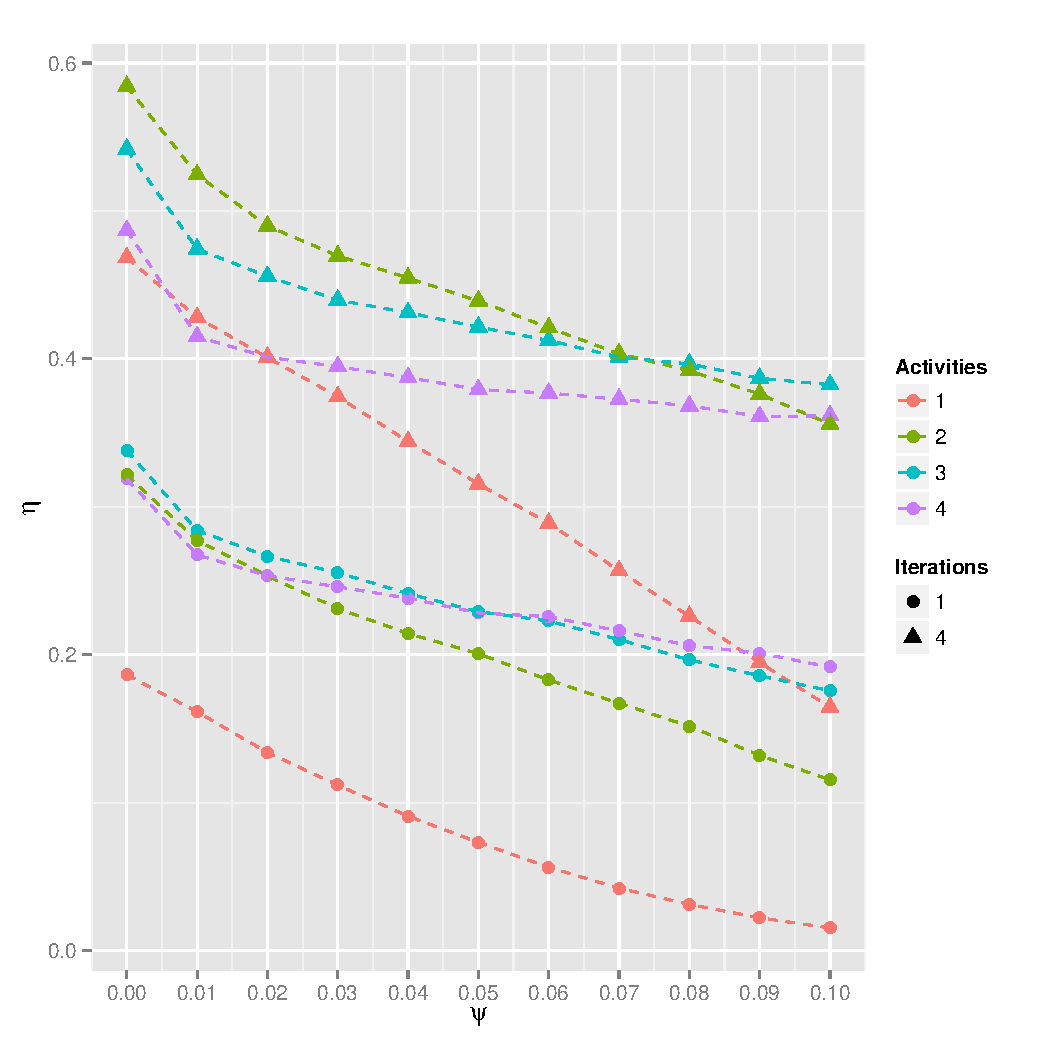
\includegraphics[scale=0.50]{Courbes/5portant_psi_c8l256e4}
		\caption{Comparison of efficiencies between different number of activities per cluster :  8 clusters, 256 neurons per cluster, 1000 sampled messages, pools of 5 networks \label{comppsi}}
	\end{figure}

	We compute values represented on figure \ref{comppsi} by scanning on the number of messages, so as to find the maximum efficiency.	
	
	After a transition, efficiencies seem to follow a linear decreasing low according to $\psi$.	
	
	Absolute values of slopes diminish for increasing number of activities per cluster. We can conclude multipartite cliques improve the resilience of the network.
	
	$\eta_{m, \psi} = P_{retrieve} m  \frac{2 \left(c \log_2{l \choose a } - \log_2(m) + 1 \right)}{c(c-1)l^2} \times (1-{l \choose a}^{c - c_e})^{-(m-1)} \times \frac{1}{1 + \psi \log_2(\psi) +(1-\psi) \log_2(1-\psi)} $
	
	$\eta_\psi = max_x \, \eta_{x, \psi}$
	
	
	Figure \ref{comppsi} seems to indicate a linear relationship (after a transition for multiple activities) between $\eta_\psi -\eta_0$ and $\psi$.
	\section{Maximum theoretical efficiency}
		It was shown in \cite{oo}, asymptotic capacities of clique networks is $\log 2$. We generalise this result to multipartite cliques.
		
		The entropy of the messages set can be approximated as $H(\mathcal{M}) \approx m c \log_2 {l \choose a}$. From $d = 1 - \left (1- \left(\frac{a}{l}\right)^2 \right)^m$, we can deduce $m \sim \frac{\log_2(1-d)}{\log_2(1-(\frac{a}{l})^2)} \sim - \frac{l^2 \log_2(1-d) \log 2}{a^2}$.
		We set $\log_2 {l \choose a} = k c$ (otherwise density approaches $0$ or $1$, and efficiency $0$). It follows that $\eta \sim c \log_2 {l \choose a} \log2(1-d) \sim \frac{k c^2 \log_2(1-d)\log 2}{a^2 {c \choose 2}}$. 
		
		$\eta \sim - 2 k  \log_2 ((1-d)a^{-2}\log 2$.
		
		We can bound the probability $P_{\exists e}$ for a message being "present" in the network, that is to mean adding it will not add any edge to the network. By union-bound $P_{\exists e} \le {l \choose a}^c d^{a^2 {c \choose 2}} = 2^{c \log_ 2 {l \choose a} + a^2 {c \choose 2 }\log_2(d)} \approx 2^{c^2(k + \frac{a^2}{2} \log_2 (d))}$.
		
		Fixing $k^* = -\frac{a^2}{2} \log_2 (d)$ gives us $\eta \sim \log_2 d \log_2 (1-d) \log 2$ and therefore \[\eta_{max} = \log 2\]
	
		Multipartite cliques don't improve theoretical efficiency (for not accepting messages that weren't previously seen by the network)

	
	\section{Conclusion}	
	
	
	
	%Marche mieux pouur de petits c --> le faire sur le sparse ?
	
	
	
	\nocite{*}
	\bibliographystyle{numeric} % Le style est mis entre crochets.
         \bibliography{bibli}
\end{document}
